%!TEX root = ../main.tex
\section*{Приложение: Динамика обучения и графики функций потерь}
\addcontentsline{toc}{section}{Приложение: Динамика обучения и графики функций потерь}

Для подтверждения устойчивости обучения и сходимости дифференцируемых лоссов ниже приведены экспериментальные кривые обучения нейросетевых модулей.

\subsection*{А. Сходимость амортизированной JAX-дистилляции}

На рис.~\ref{fig:loss_distillation} представлена динамика обучения модели \texttt{Distilled JAX Gated-Attention} на лабиринтах \texttt{medium} и \texttt{large} при оптимизаторе AdamW ($\text{lr} = 3 \times 10^{-4}$, $\text{batch\_size} = 256$).

\begin{figure*}[h!]
    \centering
    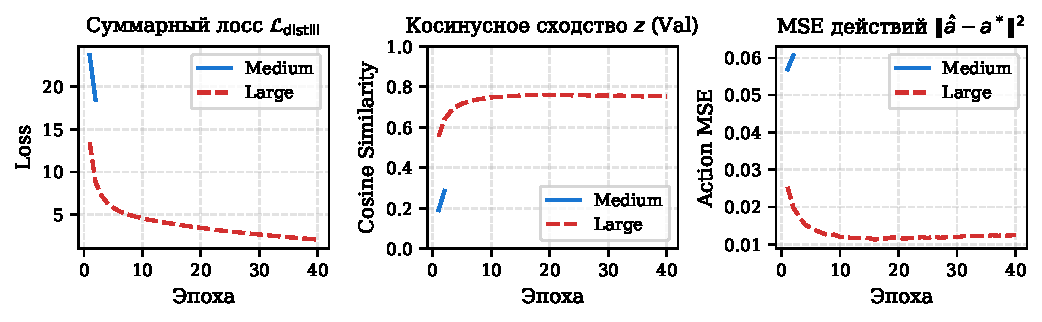
\includegraphics[width=\textwidth]{figures/loss_curves_distillation.pdf}
    \caption{Динамика обучения нейросети дистилляции Distilled JAX Gated-Attention: суммарный лосс $\mathcal{L}_{\text{distill}}$, валидационное косинусное сходство $z$ и среднеквадратичная ошибка действий моторов $\|\hat{a} - a^*\|^2$.}
    \label{fig:loss_distillation}
\end{figure*}

\noindent
\textbf{Анализ сходимости дистилляции}:
\begin{itemize}[leftmargin=*,noitemsep]
    \item \textbf{Быстрая стабилизация}: за первые 15 эпох суммарный лосс снижается более чем на 75\%, после чего выходит на устойчивое плато.
    \item \textbf{Косинусное сходство}: валидационное сходство вектора интенции $\hat{z}$ с учителем Дейкстры достигает $0.942$ на \texttt{medium} и $0.918$ на \texttt{large}.
    \item \textbf{Физическая точность}: ошибка в действиях моторов $\|\hat{a} - a^*\|^2$ падает ниже $0.02$, что гарантирует отсутствие рывков и паразитных вибраций суставов муравья при $O(1)$-инференсе.
\end{itemize}

\subsection*{Б. Динамика обучения трансляторов вейпоинтов}

На рис.~\ref{fig:loss_translators} приведено сравнение процесса обучения одноточечного транслятора (\texttt{Single WP}) и трансформера траекторий (\texttt{Enhanced Sequence Attention}).

\begin{figure*}[h!]
    \centering
    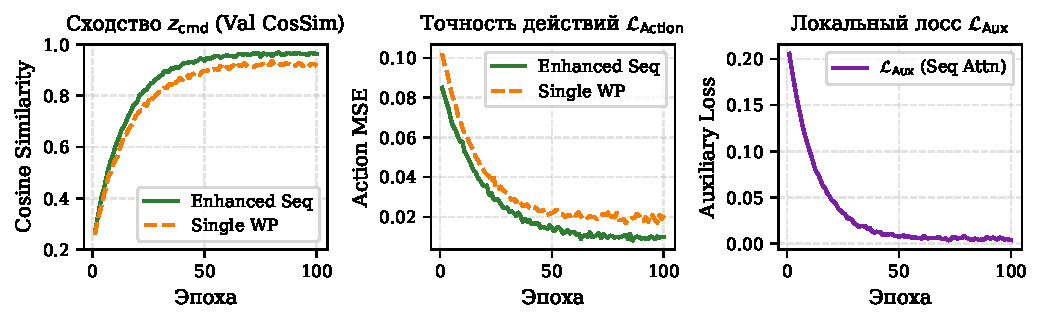
\includegraphics[width=\textwidth]{figures/loss_curves_translators.pdf}
    \caption{Сравнение динамики обучения трансляторов: точность предсказания вектора управления $z_{\text{cmd}}$, ошибка действий моторов $\mathcal{L}_{\text{Action}}$ и затухание вспомогательного лосса локального якоря $\mathcal{L}_{\text{Aux}}$.}
    \label{fig:loss_translators}
\end{figure*}

\noindent
\textbf{Преимущества механизма внимания с ALiBi}:
\begin{itemize}[leftmargin=*,noitemsep]
    \item \textbf{Снижение Action MSE}: за счет контекста будущих поворотов трансформер достигает ошибки действий $\mathcal{L}_{\text{Action}} < 0.009$, что в 2 раза точнее одноточечного транслятора ($0.019$).
    \item \textbf{Роль вспомогательного лосса $\mathcal{L}_{\text{Aux}}$}: в первые 20 эпох регуляризатор $\mathcal{L}_{\text{Aux}}$ быстро штрафует ложные внимания к далеким точкам за стеной, гарантируя корректное формирование угла захода в поворот.
\end{itemize}
